\chapter{塑闪阵列探测器分系统简介}
\section{工作原理}
\label{sec:psd_principle}
塑闪阵列探测器(以下将简称PSD)是暗物质粒子探测卫星的关键子探测器之一,它具有两个功能:一是鉴别入射重离子(Z=1~20)的种类;二是协助BGO量能器,区分电子和光子事件。

有机塑料闪烁体由于具有强的抗辐照特性、快的时间响应性、好的均匀性、长的光衰减长度、光输出高且易于加工等属性,在空间探测系统中常被用于提供系统的触发信号、能量测量及飞行时间测量。
PSD选择了\SI{10}{\milli\meter}厚的有机塑料闪烁体作为探测器介质材料,并使用光电倍增管作为读出器件。
PSD通过测量入射粒子在塑闪中的沉积能量来实现其粒子鉴别的功能,下面简要介绍一下其原理。

\subsection{重离子鉴别的原理}
粒子在物质中的能量损失与其能量有紧密的关系。
对于重带电粒子(质量大于电子),其平均能量损失率与入射粒子能量的关系如图~\ref{fig:ch2:energyloss_vs_velocity}所示。
在不同能量范围内,导致能量损失的主要相互作用并不一样,图~\ref{fig:ch2:energyloss_vs_velocity}中用竖直的带子区分不同的能损区域。
DAMPE关注的能量范围属于相对论能区,此时主要是电离能损和辐射能损占主导地位。
在中等能量范围内电离相互作用起主导作用,辐射效应可以忽略;随着能量的不断升高,辐射效应逐渐不断增强,并最终其占据主导地位。
而对于重离子来说,由于其质量较大,在DAMPE的能量范围内其辐射效应不明显,因此这里只考虑它们的电离能损。

当$0.1\lessapprox\beta\gamma\lessapprox1000$($\beta=v/c,\gamma=1/\sqrt{1-{\beta}^2}$)时,重带电粒子的电离能损可以用Bethe-Bloch方程准确描述(即图~\ref{fig:ch2:energyloss_vs_velocity}中的Bethe区)):
\begin{equation}\label{eq:beth_bloch}
-\left\langle\frac{dE}{dx}\right\rangle = Kz^2\frac{Z}{A}\frac{1}{{\beta}^2}
\left[\frac{1}{2}\ln\frac{2m_ec^2{\beta}^2{\gamma}^2T_{max}}{I^2}-{\beta}^2-\frac{\delta(\beta\gamma)}{2}\right]
\end{equation}
其中$-\left\langle\frac{dE}{dx}\right\rangle$表示的是粒子通过单位约化介质层厚度的平均电离能损,K为常数,Z、A是探测器介质的原子序数和质量数,z是入射粒子的电荷数,$m_e$是电子的静止质量,c是光速,I是为介质的电离常数(也称平均激发能,有效电离电位等),$T_{max}$为入射粒子与静止的电子碰撞时传递给电子的最大动能。
$\delta$是密度效应修正项。
如图~\ref{fig:ch2:energyloss_vs_velocity}所示,在Bethe区随着入射粒子的能量由低逐渐增高时,能量损失起初像$1/{\beta}^2$一样快速减小,然后到达一个很宽范围的极小值区域。
这个极小值区域最低点约在$\beta\gamma\approx3\sim4$附近,且与介质无关。
通常将此最小值处的电离能损称为最小电离,把能量损失率为最小值的粒子称为最小电离粒子(Minimum Ionizing Particles,简称MIPs)。
在高能物理中,MIPs粒子常用来统称$z=1$的相对论性粒子(如宇宙线$\mu$子),因为它们的能量损失率与最小电离值非常接近。
经过最小电离值之后($\beta\gamma>4$),能量损失率开始缓慢上升,这是由于公式~\ref{eq:beth_bloch}方括号内第一项随$\ln{\beta}^2{\gamma}^2$变大,这个过程被称为相对论性上升。
随着能量的进一步升高,入射粒子的横向电场增强,靶核核外电子电荷密度的屏蔽效应也逐渐显著,减小了能量损失率,这种效应被称为密度效应。
密度效应在公式~\ref{eq:beth_bloch}中用$\delta/2$来表示,它使得电离能量损失率减缓并最终接近一个常数值,称为费米坪(见图~\ref{fig:ch2:fermi_plateau})。

\begin{figure}
	\centering
	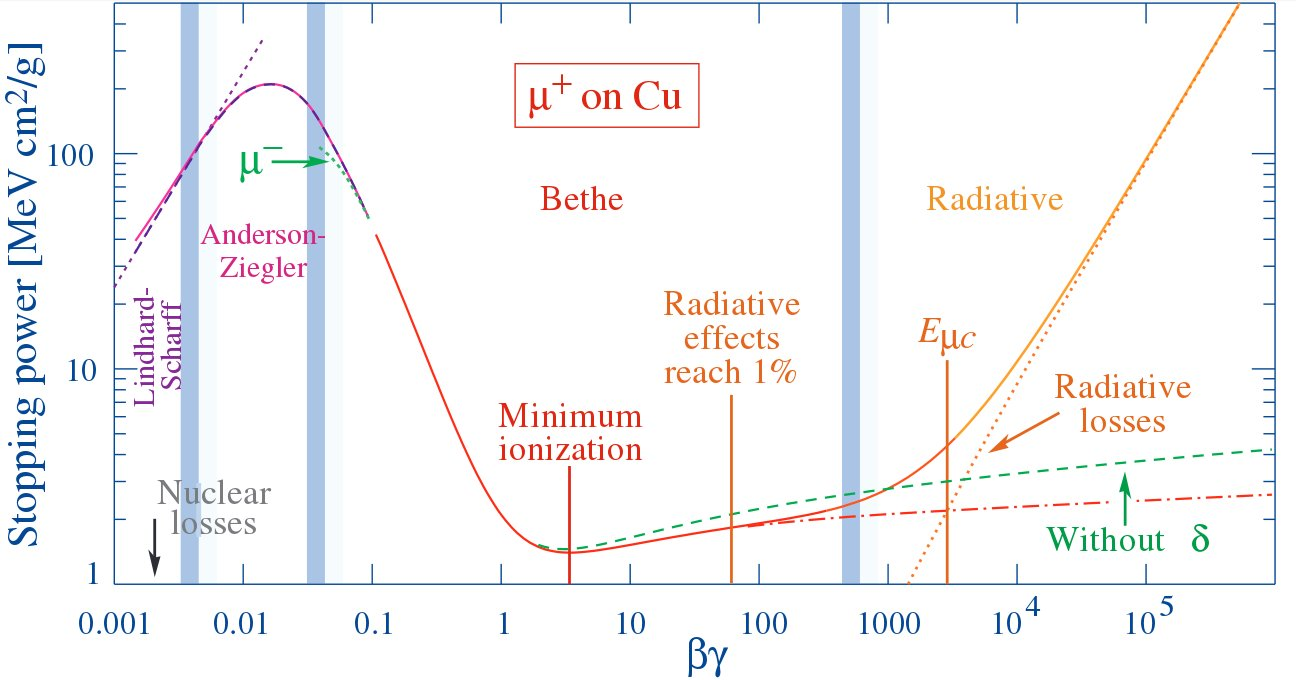
\includegraphics[width=0.8\linewidth]{chap/description/fig/energyloss_vs_velocity}
	\caption{${\mu}^+$在Cu中的能量损失率与速度的关系(用$\beta\gamma$表示),引自~\parencite{pdg_book}。 图中实线是总的能量损失率,包含了所有相互作用。}
	\label{fig:ch2:energyloss_vs_velocity}
\end{figure}

\begin{figure}
\centering
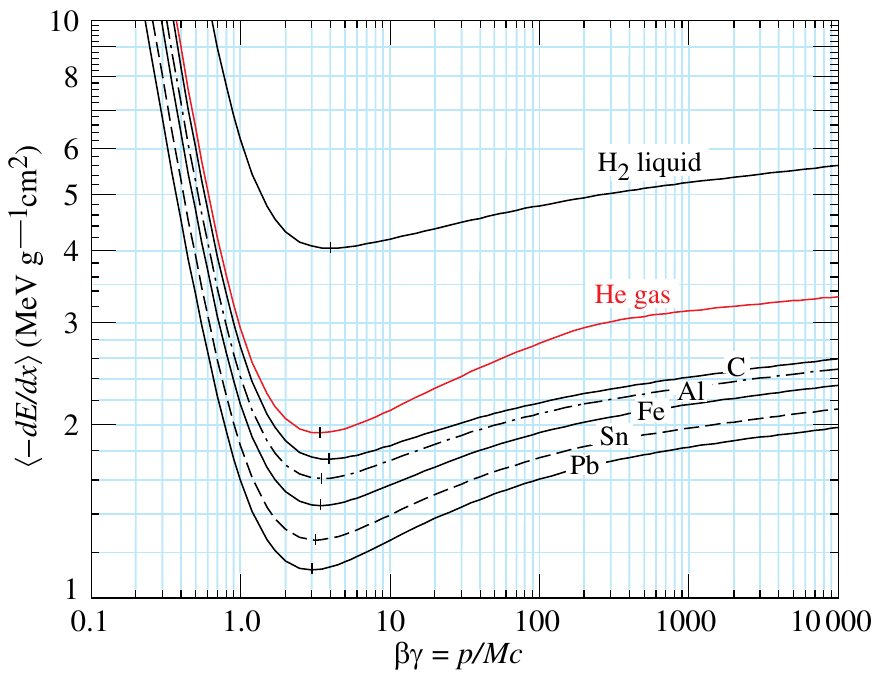
\includegraphics[width=0.8\linewidth]{chap/description/fig/fermi_plateau}
\caption{入射粒子在几种不同介质中的电离能量损失随入射粒子动量的变化,可以清楚地看到费米坪。引自~\parencite{pdg_book}。}
\label{fig:ch2:fermi_plateau}
\end{figure}

由公式~\ref{eq:beth_bloch}可知,对同一种探测介质来说,$dE/dx$只与入射粒子的电荷量$z$和速度$\beta$有关。
对于相对论粒子来说($\beta\gamma>1$),其电离能量损失虽然与速度相关,但在很大的能量范围内其变化并不大。
因此,相对论重离子的电离能损主要取决于所带电荷量,并可以近似为:
\begin{equation}
-\left\langle\frac{dE}{dx}\right\rangle \propto z^2
\end{equation}
即与电荷量的平方成正比。
由此可见,不同种类的核素在探测器介质中的电离能损相差巨大,对于塑料闪烁体材料也一样。
因此可以通过测量PSD中沉积能量的大小进行重离子的鉴别。

\subsection{高能$e/\gamma$鉴别的原理}
光子可以与物质发生多种相互作用,如图~\ref{fig:ch2:photon_energyloss}所示。
其中${\sigma}_{p.e.}$是光电效应的反应截面,
${\sigma}_{Rayleigh}$是Rayleigh散射的反应截面, 
${\sigma}_{Compton}$是康普顿散射的反应截面,
${\kappa}_{nuc}$是靶核电场导致的电子对效应的反应截面,
${\kappa}_e$是靶核核外电子电场导致的电子对效应的反应截面,
${\sigma}_{g.d.r}$是光致核反应的反应截面。
在光子能量较低时光电效应占主导作用,中等能量时康普顿散射占主导作用,而高能光子一般只通过电子对效应损失能量.
从图~\ref{fig:ch2:photon_energyloss}中可以看到电子对效应的反应截面非常小,再加上PSD使用的塑料闪烁体材料密度小、厚度薄,高能$\gamma$射线在PSD中发生反应的概率非常小,因此基本不会有能量沉积。

\begin{figure}[t]
	\centering
	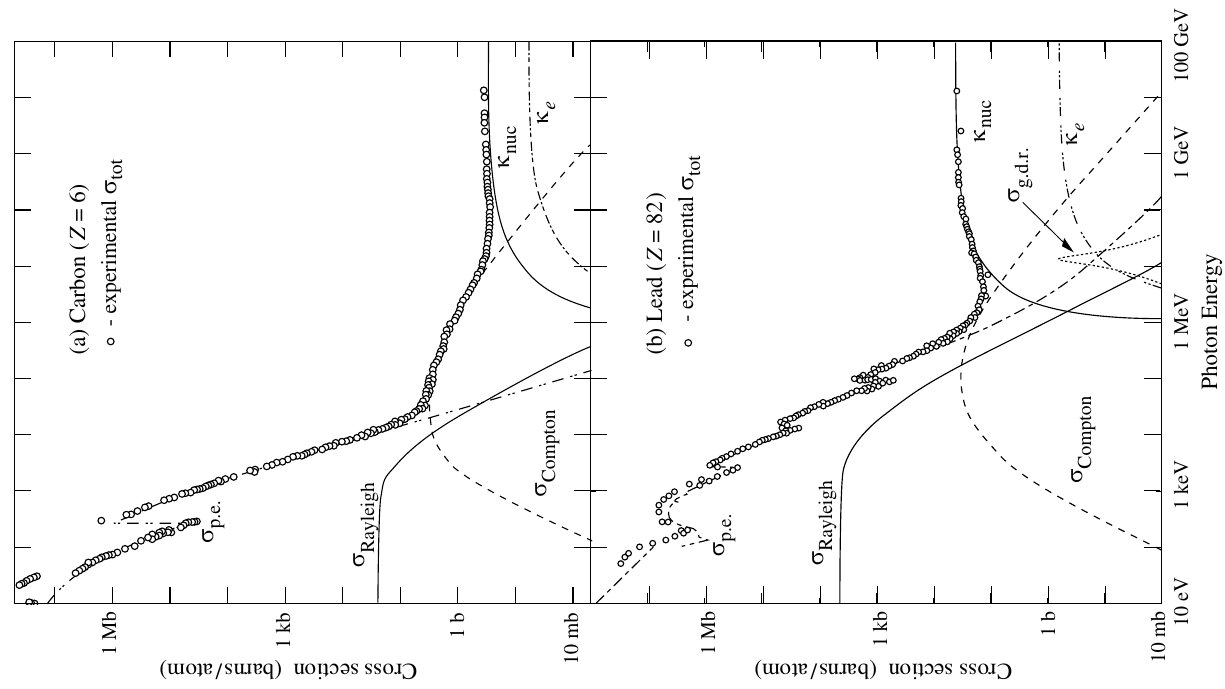
\includegraphics[width=0.9\linewidth,angle=270]{chap/description/fig/photon_energyloss}
	\caption{光子与物质各种相互作用的反应截面,上图是在碳中的,下图是在铅中的,引自~\parencite{pdg_book}。}
	\label{fig:ch2:photon_energyloss}
\end{figure}

对于电子/正电子来说,它们的质量小,在物质中的能量损失情况与重带电粒子有很大的不同。
电子/正电子与靶原子的相互作用,主要是电离能量损失,辐射能量损失和多次散射。
在能量较低时,电子/正电子虽然可以通过Møller散射,Bhabha散射和正电子湮灭损失能量,但电离能损仍然占据主导地位,见图~\ref{fig:ch2:electron_energyloss}。
随着电子/正电子能量的升高,轫致辐射效应开始显著起来,并随着能量的增大近似以线性形式增强。
电离能损随着能量的增大以对数形式增强,因此当能量大于\SI{100}{MeV}之后轫致辐射导致的能损开始占据主导地位。
在DAMPE关注的能区,穿过PSD的电子/正电子主要通过轫致辐射损失能量。
然而,高能电子/正电子轫致辐射产生的光子能量也比较高,一般不在PSD中沉积能量。
另一方面,电离相互作用虽然不占据主导作用,但它是一个连续过程,会一直在PSD中沉积能量,其大小大概与MIPs粒子的能量沉积差不多。

\begin{figure}
\centering
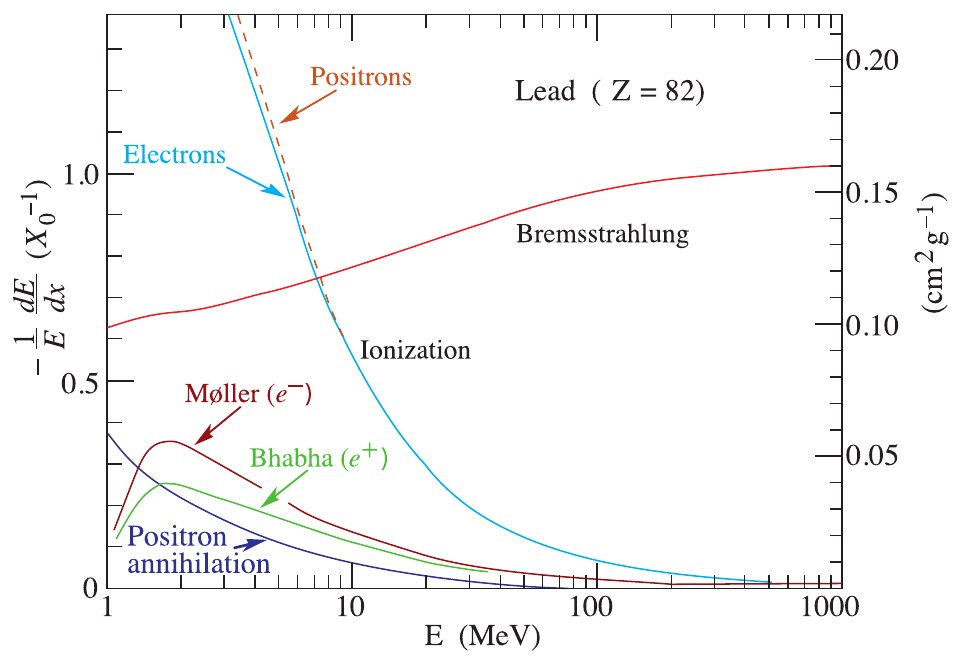
\includegraphics[width=0.8\linewidth]{chap/description/fig/electron_energyloss}
\caption{电子/正电子在铅中的单位辐射长度能损比例与能量的关系,引自~\parencite{pdg_book}。}
\label{fig:ch2:electron_energyloss}
\end{figure}

综上所述,高能光子在PSD中没有能量沉积,高能电子/正电子在PSD中有能量沉积。
根据入射粒子是否在PSD中有能量沉积,可以将光子和带电粒子区分开来;进一步结合BGO量能器,可以将电子/正电子和其它带电的强子区分开来。

\section{性能要求}
\label{sec:psd_requirements}
结合DAMPE探测器整体的物理需求,PSD需要达到的性能指标如下:
\begin{enumerate}
	\item 有效探测面积$\SI{820}{\milli\meter}\times\SI{820}{\milli\meter}$。DAMPE是单方向的探测器,即它只关心从顶部入射的粒子。由于PSD位于DAMPE探测器最顶端,它的有效探测面积决定了DAMPE的视场大小。PSD是DAMPE中面积最大的子探测器。
	\item 探测单元实现电子和重离子($Z=1\sim20$)的测量。根据~\ref{sec:psd_principle}节的描述,重离子在PSD中的能量沉积相差巨大,这就对PSD探测单元提出了大动态范围的要求。另外,为了有效区分电子信号和噪声本底(光子不在PSD中产生信号),探测单元还需要由较高的信噪比(Signal to Noise Ratio,简称SNR)。因此PSD的探测单元需要进行认真地设计和验证以满足这些要求,这将在第三章进行详细讨论。
	\item 探测单元电荷分辨优于\SI{25}{\percent}($\sigma$,Z=1)。为了对不同种类的重离子进行有效鉴别,探测器分辨率需要满足一定条件。由于塑料闪烁体材料本身的限制,PSD探测探测单元的分辨率确定为对$Z=1$的粒子(对于$Z>1$的重离子,探测器响应很难在实验室条件下进行验证)的$\sigma$好于\SI{25}{\percent}。在相对论能区,所有$Z=1$的粒子与MIPs粒子具有类似的能量沉积,这个要求可以简化为对MIPs粒子的能量分辨好于\SI{25}{\percent}。
	\item 空间分辨好于\SI{2}{\centi\meter}。迳迹探测不是PSD的主要功能,DAMPE的主要迳迹探测器是STK。但在迳迹寻找和重建过程中,STK需要BGO和PSD提供额外的位置信息以便其更有效地找到并验证真实迳迹。因此,PSD的位置信息不需要特别精确,最终被确定为\SI{2}{\centi\meter}。
	\item 对MIPs粒子的探测效率高于\SI{95}{\percent}。这是$e/\gamma$鉴别提出的要求,包含两部分内容:一是对带电粒子的探测器效率高于\SI{95}{\percent},二是对光子的误判率低于\SI{5}{\percent}。
\end{enumerate}

\section{探测器设计和组成}
\label{sec:psd_composition}
入射粒子在BGO量能器中发生电磁簇射或强子簇射时,大部分次级粒子都是前向的,但也有小部分次级粒子由于大角度散射反照(backscatter)到PSD上。
反散射的簇射粒子由于带电或能量较低,在PSD上会有能量沉积,使得PSD测到的能量变大,这可能造成光子被误判为带电粒子,或者质子被误判为重离子。
为了减小由此引起的误判率,PSD采用了模块化设计,即将PSD切割成一个个足够小的探测单元。
反散射粒子在入射粒子迳迹周围会有一个分布,且在入射粒子穿过的PSD探测单元内接收的反散射粒子最少(因为\ang{180}反散射的概率最小)。
如果只使用入射粒子穿过的PSD探测单元作为粒子鉴别的依据,就可以大大降低反散射簇射粒子造成的误判率。
由于每个探测单元有对应一个固定的位置,PSD模块化带来的另一个好处是增加了一组位置信息。

PSD探测器的整体构型如图~\ref{fig:ch2:psd_explosion}所示。
每层塑闪阵列内由41根塑闪单元条组成。
每个探测单元模块由一根塑闪单元条,两端耦合光电倍增管组成


\begin{figure}
\centering
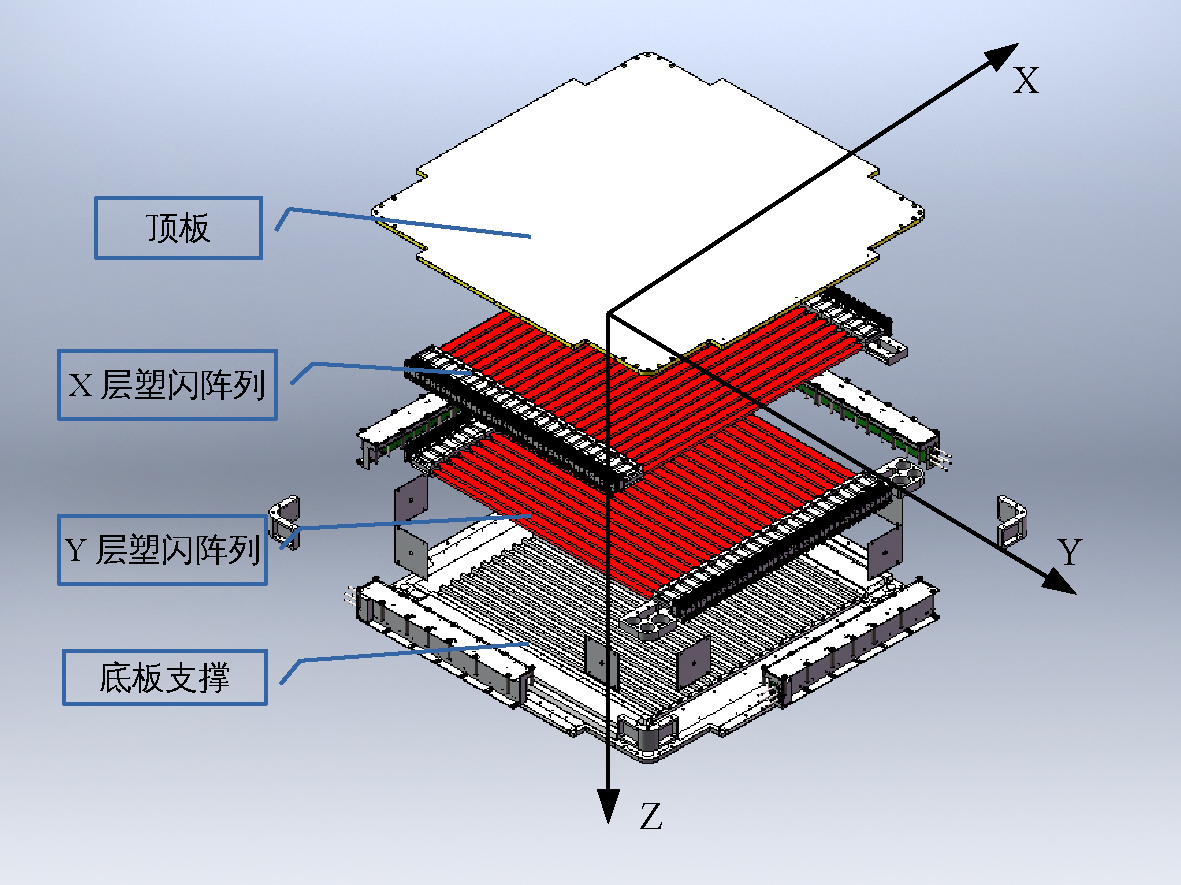
\includegraphics[width=0.8\linewidth]{chap/description/fig/psd_explosion}
\caption{PSD探测器结构的爆炸图展示。}
\label{fig:ch2:psd_explosion}
\end{figure}


PSD选择了Eljeng公司的EJ-200~\parencite{ej-200}作为探测器介质材料,其主要性能参数参看表~\ref{tab:ch2:ej200}。


\begin{longtabu} to 0.8\linewidth{lX}
	\caption{EJ-200的主要性能参数\label{tab:ch2:ej200}}\\
	\toprule[1.5pt]
	\textbf{性能参数} & \textbf{典型值} \\ 
	\midrule
	\endfirsthead
	
	%\toprule[1.5pt]
	\multicolumn{2}{ c }{续表~\ref{tab:ch2:ej200}}\\
	%性能参数 & 典型值 \\ 
	\midrule
	\endhead
	
	%\bottomrule[1.5pt]
	\endfoot
	
	\bottomrule[1.5pt]
	\endlastfoot
	
	H/C原子比 & 1.10 \\
	原子密度 & H: \SI{5.523E22}{\per\cubic\centi\meter}, C:\SI{4.740E22}{\per\cubic\centi\meter} \\
	光输出 & \SI{64}{\percent}(相对蒽)\footnote{\SI{60}{\celsius}时的光输出是\SI{20}{\celsius}时的\SI{95}{\percent},\SI{-60}{\celsius}$\sim$\SI{20}{\celsius}时光输出不依赖于温度} \\
	上升时间 & \SI{0.9}{\nano\second} \\
	衰减时间 & \SI{2.1}{\nano\second} \\
	光谱峰位 & \SI{425}{\nano\meter} \\
	衰减长度 & \SI{210}{\centi\meter} \\
	折射率   & 1.58 \\
	密度    &  \SI{1.032}{\g\per\cubic\centi\meter} \\
	膨胀系数 & \SI{7.8E-5}{\per\celsius} \\
	软化温度 & \SI{70}{\celsius} \\
	蒸气压   & 能用于真空 \\
	溶解性  &  可溶于芳香族溶剂、氯化溶剂及丙酮等,不溶于水、稀酸、低浓度酒精、碱及硅脂等 \\
\end{longtabu}

\begin{longtabu} to 0.6\linewidth{lX}
	\caption{R4443 Mod2的主要性能参数\label{tab:ch2:r4443}}\\
	\toprule[1.5pt]
	\textbf{性能参数} & \textbf{典型值} \\ 
	\midrule
	\endfirsthead
	
	%\toprule[1.5pt]
	\multicolumn{2}{ c }{续表~\ref{tab:ch2:ej200}}\\
	%性能参数 & 典型值 \\ 
	\midrule
	\endhead
	
	%\bottomrule[1.5pt]
	\endfoot
	
	\bottomrule[1.5pt]
	\endlastfoot
	
	波长响应范围 & 300$\sim$650 \si{\nano\meter} \\
	光谱峰位 & \SI{375}{\nano\meter} \\
	光阴极材料 & 低噪声双碱金属 \\
	光阴极最小有效面积 & \SI{10}{\milli\meter} \\
	工作温度 & \SI{-30}{\celsius}$\sim$\SI{50}{\celsius} \\
	上升时间 & \SI{2.5}{\nano\second} \\
	渡越时间 & \SI{24}{\nano\second} \\
	打拿极数 & 10 \\
	典型增益 & \SI{1.0E6}{} \\
	最大工作电压 & \SI{1250}{\volt}\\
	重量 & \SI{11}{\g}\\
	外部尺寸(直径) & \num[separate-uncertainty]{14.5(7)} \si{\milli\meter} \\
	典型暗电流 & \SI{0.5}{\nano\ampere}\\
	最大暗电流 & \SI{4.0}{\nano\ampere} \\
	冲击 & \SI{5000}{\meter\per\square\second}(500 g's)\\
	振动 & \SI{200}{\meter\per\square\second}(20 g's) \\ 
\end{longtabu}

\begin{table}[htb]
	\centering
	\caption{EJ-560主要性能参数}
	\label{tab:ch2:ej560}

		\begin{tabulary}{0.6\linewidth}{LC}
			\toprule[1.5pt]
			\textbf{物理性能} & \textbf{典型值}  \\ 
			\midrule[1pt]
			厚度 & \SI{3}{\milli\meter} \\
			密度 & \SI{1.03}{\g\per\cubic\centi\meter} \\
			硬度(A型邵氏硬度计) & 16$\sim$24 \\
			折射率 & 1.43 \\
			工作温度范围 & \SI{-40}{\celsius}$\sim$\SI{70}{\celsius} \\
			热膨胀系数 & \SI{3E-4}{\per\celsius}\\		
			\bottomrule[1.5pt] 
		\end{tabulary}

\end{table}

\begin{figure}
\centering
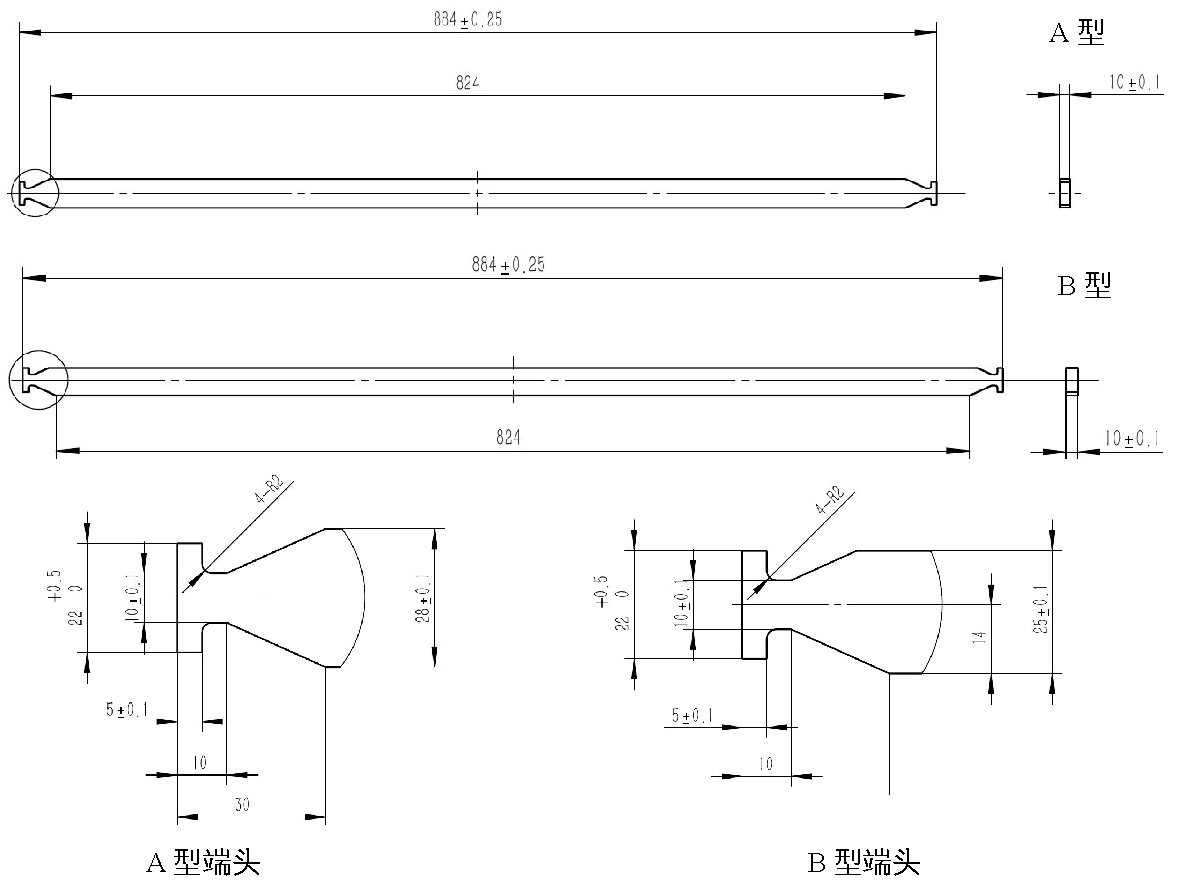
\includegraphics[width=\linewidth]{chap/description/fig/bars}
\caption{PSD中两种塑闪单元条的尺寸}
\label{fig:ch2:bars}
\end{figure}

\begin{figure}
\centering
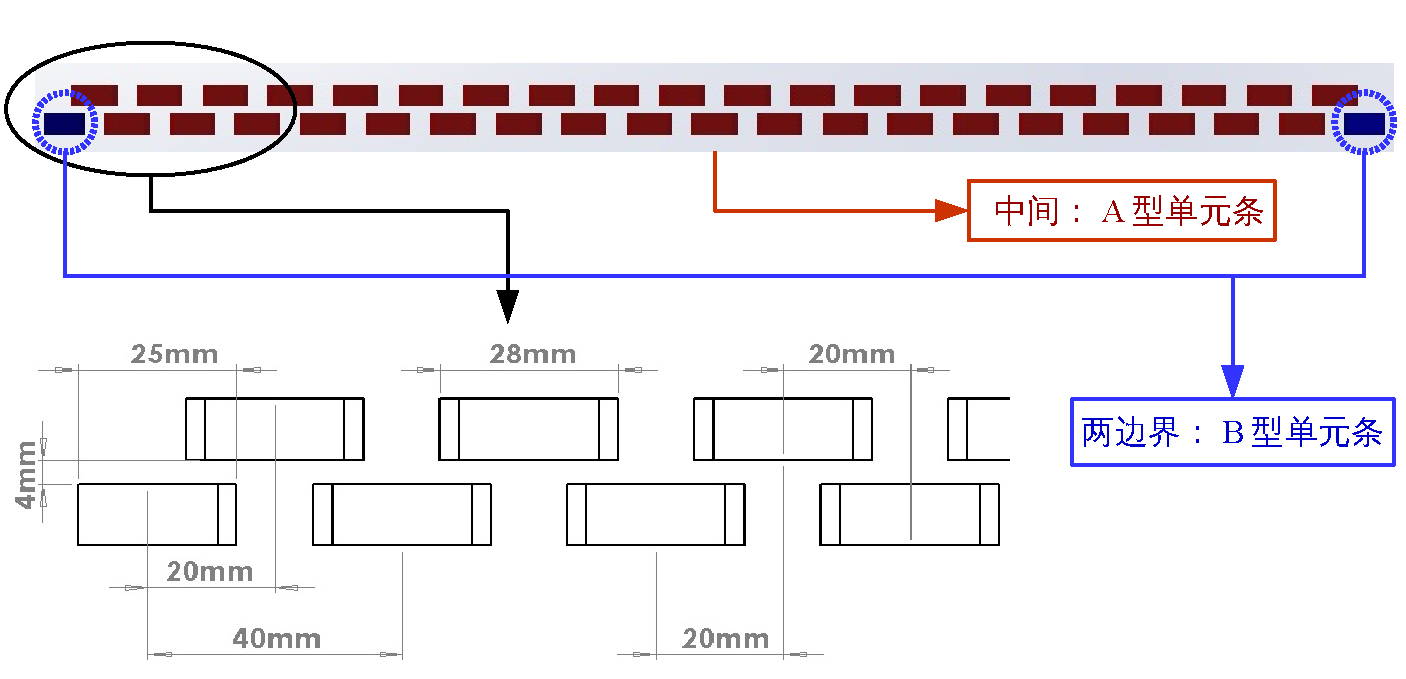
\includegraphics[width=1\linewidth]{chap/description/fig/bars_layout}
\caption{PSD每一塑闪层内的单元条交叠放置以消除探测器灵敏死区。}
\label{fig:ch2:bars_layout}
\end{figure}

\section{前端电子学}
\label{sec:psd_electronics}
\begin{figure}[t]
\centering
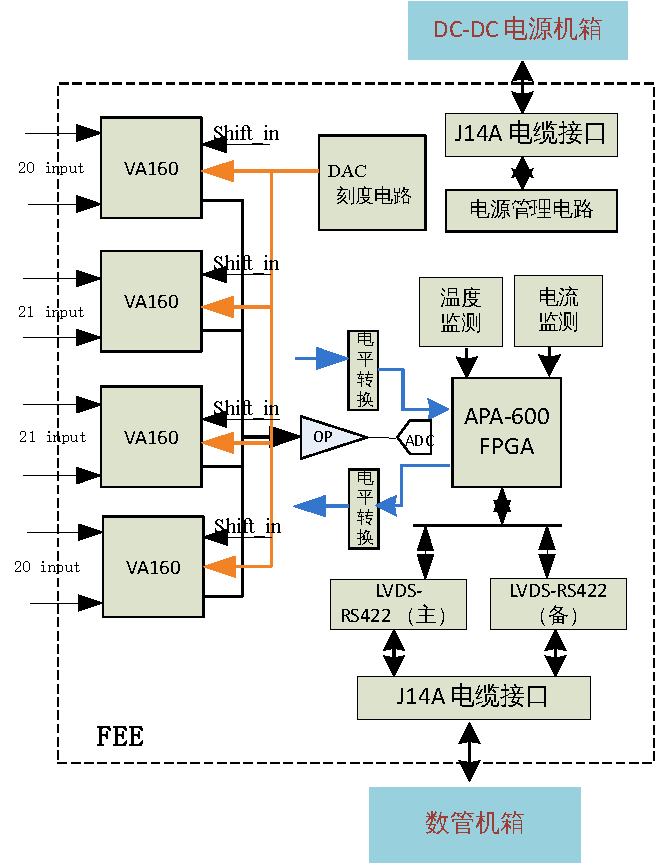
\includegraphics[width=0.8\linewidth]{chap/description/fig/psd_fee1}
\caption{PSD的前端电子学原理框图。}
\label{fig:ch2:psd_fee1}
\end{figure}

\begin{figure}
\centering
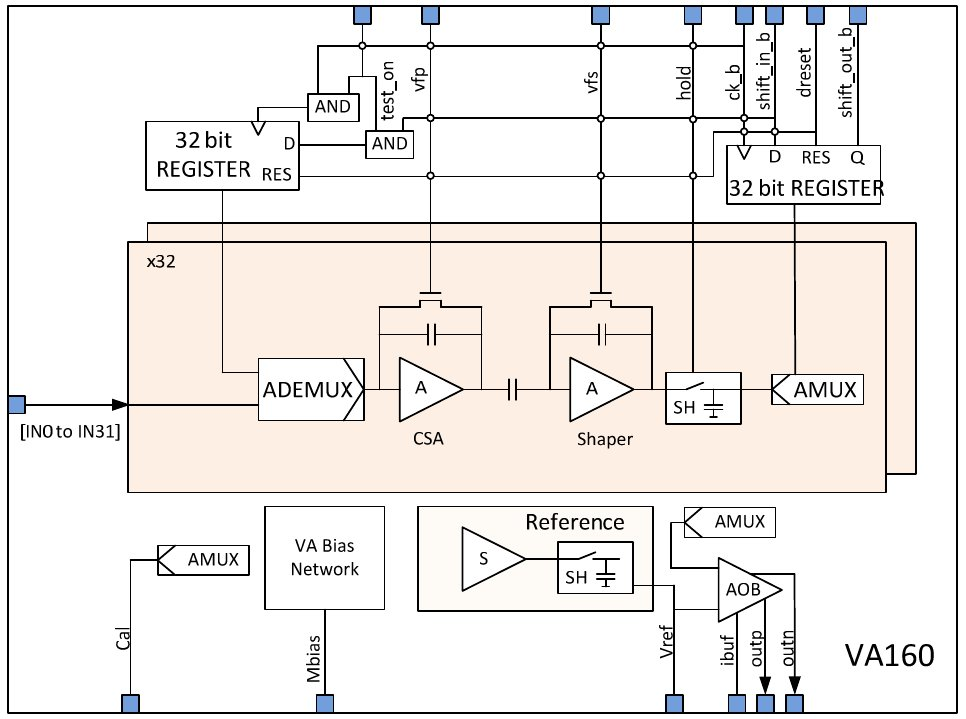
\includegraphics[width=0.8\linewidth]{chap/description/fig/va160}
\caption{VA160原理框图}
\label{fig:ch2:va160}
\end{figure}

\section{支撑结构}
\label{sec:psd_support}